\documentclass{article}
\usepackage[utf8]{inputenc}
\usepackage{graphicx}
\usepackage{float}
\usepackage{geometry}
\geometry{a4paper, margin=1in}

\title{Relatório do Projeto: Solar Tracker}
\author{Igor Cleto e Matheus Galbiatti}
\date{Belo Horizonte, 10 de julho de 2025}

\begin{document}

\begin{titlepage}
    \centering
    
\includegraphics[width=0.4\textwidth]{logo_ufmg.png} % Placeholder for UFMG logo
    \vspace{1cm}
    
    {\huge\bfseries Universidade Federal de Minas Gerais}
    \vspace{1cm}
    
    {\Large\bfseries Escola de Engenharia}
    \vspace{1.5cm}
    
    {\Large\bfseries Disciplina: Projeto de Sistemas Embutidos}
    \vspace{2cm}
    
    {\Huge\bfseries Relatório do Projeto: Solar Tracker}
    \vspace{2cm}
    
    {\large\bfseries Autores:}
    
    {\large Igor Cleto}
    
    {\large Matheus Galbiatti}
    
    \vfill
    
    {\large Belo Horizonte}
    
    {\large 10 de julho de 2025}
\end{titlepage}

\tableofcontents
\newpage

\section{Introdução}
Este documento detalha o projeto e desenvolvimento de um protótipo de rastreador solar de eixo único (azimutal), concebido no âmbito da disciplina de Projeto de Sistemas Embutidos. O objetivo principal é criar uma solução de baixo custo e autossustentável para otimizar a captação de energia solar, abordando a limitação de eficiência dos painéis solares fixos. O projeto foi planejado utilizando a metodologia do Project Model Canvas para estruturar as ideias e garantir o alinhamento entre os objetivos, requisitos e restrições.

\section{Project Model Canvas}
O Project Model Canvas é uma ferramenta de gerenciamento visual utilizada para descrever, projetar e analisar modelos de projetos de forma concisa e integrada. Ele é composto por 13 blocos que cobrem as áreas fundamentais de um projeto, desde suas justificativas e objetivos até os custos e cronograma. A seguir, cada um dos blocos é detalhado conforme definido para o projeto Solar Tracker.

\subsection{Justificativas}
Painéis solares fixos apresentam uma limitação intrínseca na captação de energia, pois não acompanham o movimento aparente do sol, resultando em menor eficiência ao longo do dia.

\subsection{Produto}
Sistema de otimização para a captação de energia solar, que opera por meio do acompanhamento do azimute solar, sendo complementado pela documentação técnica.

\subsection{Objetivo SMART}
Desenvolver um protótipo funcional de um sistema de rastreamento solar de eixo único (azimutal) para aumentar a captação de energia de um painel solar de maneira autossustentável.

\subsection{Requisitos}
\begin{itemize}
    \item \textbf{Rastreamento Solar Autônomo:} Detectar e seguir autonomamente a luz solar.
    \item \textbf{Movimentação:} Em um eixo (azimutal).
    \item \textbf{Simplicidade:} Componentes de hardware e software simples, com uma interface de usuário (IU) intuitiva.
    \item \textbf{Desempenho Operacional:} Operação confiável e ágil.
    \item \textbf{Restrição Orçamentária:} Desenvolvimento e operação dentro de um orçamento limitado.
\end{itemize}

\subsection{Benefícios Futuros}
O produto aprimora a eficiência energética e otimiza a utilização do espaço, enquanto o monitoramento remoto e uma solução de rastreamento solar de baixo custo complementam seus benefícios. O resultado é a otimização da eficiência, atendendo à necessidade de soluções energéticas práticas e eficazes.

\subsection{Stakeholders e Fatores Externos}
O projeto é influenciado por fornecedores de componentes eletrônicos e mecânicos (disponibilidade e preço), o ambiente climático (condições para testes) e potenciais usuários/avaliadores de protótipos na área de energia solar.

\subsection{Equipe}
\begin{itemize}
    \item Igor Cleto: Validação do projeto.
    \item Matheus Galbiatti: Desenvolvimento do projeto.
\end{itemize}

\subsection{Premissas}
\begin{itemize}
    \item Disponibilidade contínua dos componentes críticos no mercado.
    \item Condições de insolação solar consistentes e adequadas durante a fase de testes.
    \item Viabilidade de um design de sistema que assegure um consumo energético inferior ao ganho obtido pela captação solar.
\end{itemize}

\subsection{Riscos}
\begin{itemize}
    \item Indisponibilidade de componentes críticos.
    \item Potenciais atrasos no cronograma estabelecido de 8 semanas.
    \item Condições climáticas desfavoráveis que prejudiquem os testes planejados.
    \item Consumo energético do sistema que supere os benefícios da captação solar.
\end{itemize}

\subsection{Grupo de Entregas}
\begin{enumerate}
    \item Design e planejamento detalhado.
    \item Desenvolvimento do protótipo de hardware e software.
    \item Testes e refinamentos.
    \item Protótipo funcional e documentação final.
\end{enumerate}

\subsection{Linha do Tempo}
\begin{itemize}
    \item \textbf{Semanas 1 e 2:} Design e planejamento.
    \item \textbf{Semanas 3 a 5:} Desenvolvimento do protótipo.
    \item \textbf{Semanas 6 e 7:} Testes e refinamentos.
    \item \textbf{Semana 8:} Finalização.
\end{itemize}

\subsection{Custos}
O projeto conta com um orçamento fixo de R\$300,00, destinado exclusivamente aos componentes eletrônicos e mecânicos necessários para o protótipo.

\subsection{Restrições}
\begin{itemize}
    \item Testes do protótipo excluem condições climáticas extremas.
    \item Os membros da equipe vão dedicar 5 horas por semana para o desenvolvimento e acompanhamento do projeto.
\end{itemize}

\section{Hardware e Componentes}
% Conteúdo a ser adicionado futuramente.

\section{Backend}
% Conteúdo a ser adicionado futuramente.

\section{Frontend com Streamlit}
O frontend do projeto é um dashboard interativo desenvolvido integralmente em Python com a biblioteca Streamlit. A escolha desta tecnologia foi estratégica, visando acelerar o ciclo de desenvolvimento ao eliminar a necessidade de linguagens de frontend tradicionais (HTML, CSS, JavaScript) e facilitar a integração direta com a lógica de controle e análise de dados do projeto.

\subsection{Arquitetura e Fluxo de Dados}
A aplicação Streamlit atua como o centro de controle e monitoramento do Solar Tracker. Sua arquitetura é baseada em um fluxo de dados em tempo real, sustentado por quatro tecnologias principais.

\begin{itemize}
    \item \textbf{Streamlit:} É o framework que renderiza a interface web. Para garantir que a interface reflita os dados mais recentes, a biblioteca \texttt{streamlit-autorefresh} é utilizada para recarregar a página a cada 500 milissegundos.
    \item \textbf{Paho-MQTT:} A comunicação com o hardware (ESP32) é desacoplada e realizada através do protocolo MQTT. A aplicação se conecta a um broker EMQX Cloud e opera de duas formas:
    \begin{itemize}
        \item \textbf{Subscrição:} Inscreve-se no tópico \texttt{esp32/angulo} para receber, de forma assíncrona, as atualizações de estado do painel. O payload esperado é uma string no formato \texttt{"angulo;azimute;manual;rele"}.
        \item \textbf{Publicação:} Publica mensagens no tópico \texttt{esp32/comando} para enviar instruções ao microcontrolador, como a mudança de modo de operação ou a definição de um ângulo manual.
    \end{itemize}
    \item \textbf{Pandas:} É utilizado para a gestão dos dados históricos. Cada mensagem recebida via MQTT é processada e salva como uma nova linha em um arquivo CSV (\texttt{dados\_historicos.csv}), que armazena o timestamp, ângulo, azimute, modo manual e estado do relé. Isso garante a persistência dos dados.
\end{itemize}

\subsection{Gestão de Estado e Atualização da Interface}
A gestão de estado é crucial em aplicações Streamlit. O objeto \texttt{st.session\_state} é utilizado para manter a persistência de dados e conexões durante a sessão do usuário:
\begin{itemize}
    \item \texttt{st.session\_state.mqtt\_client}: Armazena a instância do cliente MQTT, garantindo que a conexão com o broker seja estabelecida apenas uma vez.
    \item \texttt{st.session\_state.dados\_atuais}: Um dicionário que guarda os dados mais recentes lidos do arquivo CSV, permitindo que sejam exibidos na interface.
    \item \texttt{st.session\_state.historico}: Mantém o DataFrame do Pandas com todos os dados históricos.
    \item \texttt{st.session\_state.operating\_mode}: Armazena o modo de operação selecionado pelo usuário (Manual ou Automático).
\end{itemize}
A comunicação MQTT é tratada de forma assíncrona com \texttt{client.loop\_start()}, que cria um thread em segundo plano. A função de callback \texttt{on\_message} é responsável por receber os dados, processá-los e anexá-los ao arquivo CSV. A interface do Streamlit, por sua vez, é atualizada através do mecanismo de auto-refresh, que aciona uma função para recarregar os dados do CSV e redesenhar os componentes da tela com as informações mais recentes.

\subsection{Detalhes da Interface de Usuário}
A interface foi projetada para ser clara e funcional, dividida em um painel de controle e um dashboard principal.

\subsubsection{Painel de Controle (Sidebar)}
A barra lateral (\texttt{st.sidebar}) agrupa os controles interativos:
\begin{itemize}
    \item \textbf{Modo de Operação:} Dois botões distintos (\texttt{st.button}), "Ativar Modo Automático" e "Ativar Modo Manual", permitem ao usuário alternar entre os modos. O estado do botão é desativado se o modo correspondente já estiver ativo, fornecendo um feedback visual claro. Ao clicar, um comando ('A' para automático, 'M' para manual) é publicado no tópico MQTT.
    \item \textbf{Controle Manual:} Visível apenas no modo "Manual", este controle utiliza um \texttt{st.slider} para uma seleção de ângulo intuitiva (0 a 180 graus). O comando só é enviado ao clicar no botão "Enviar Ângulo", evitando o envio contínuo de mensagens MQTT.
\end{itemize}

\subsubsection{Dashboard Principal}
A área principal foca na visualização dos dados em tempo real e histórico:
\begin{itemize}
    \item \textbf{Status Atual:} Quatro métricas principais são exibidas usando \texttt{st.columns} para organização.
    \begin{itemize}
        \item \textbf{Ângulo e Azimute:} Componentes \texttt{st.metric} mostram os valores numéricos atuais.
        \item \textbf{Modo e Relé:} Para o modo de operação e o estado do relé, foi utilizado HTML personalizado dentro de \texttt{st.markdown} para criar indicadores visuais (LEDs) que mudam de cor (verde para ativo/ligado, vermelho para inativo/desligado), oferecendo um feedback rápido e intuitivo.
    \end{itemize}
    \item \textbf{Gráfico Histórico:} O \texttt{st.line\_chart} renderiza o histórico de ângulos e azimutes, utilizando o timestamp como índice para o eixo X.
    \item \textbf{Tabela de Dados:} O uso do \texttt{st.expander} permite que o usuário visualize a tabela completa de dados históricos (\texttt{st.dataframe}), mantendo a interface principal limpa e organizada.
\end{itemize}

As figuras \ref{fig:tela_automatico} e \ref{fig:tela_manual} ilustram a aparência do dashboard em seus dois modos de operação principais.

\begin{figure}[H]
    \centering
    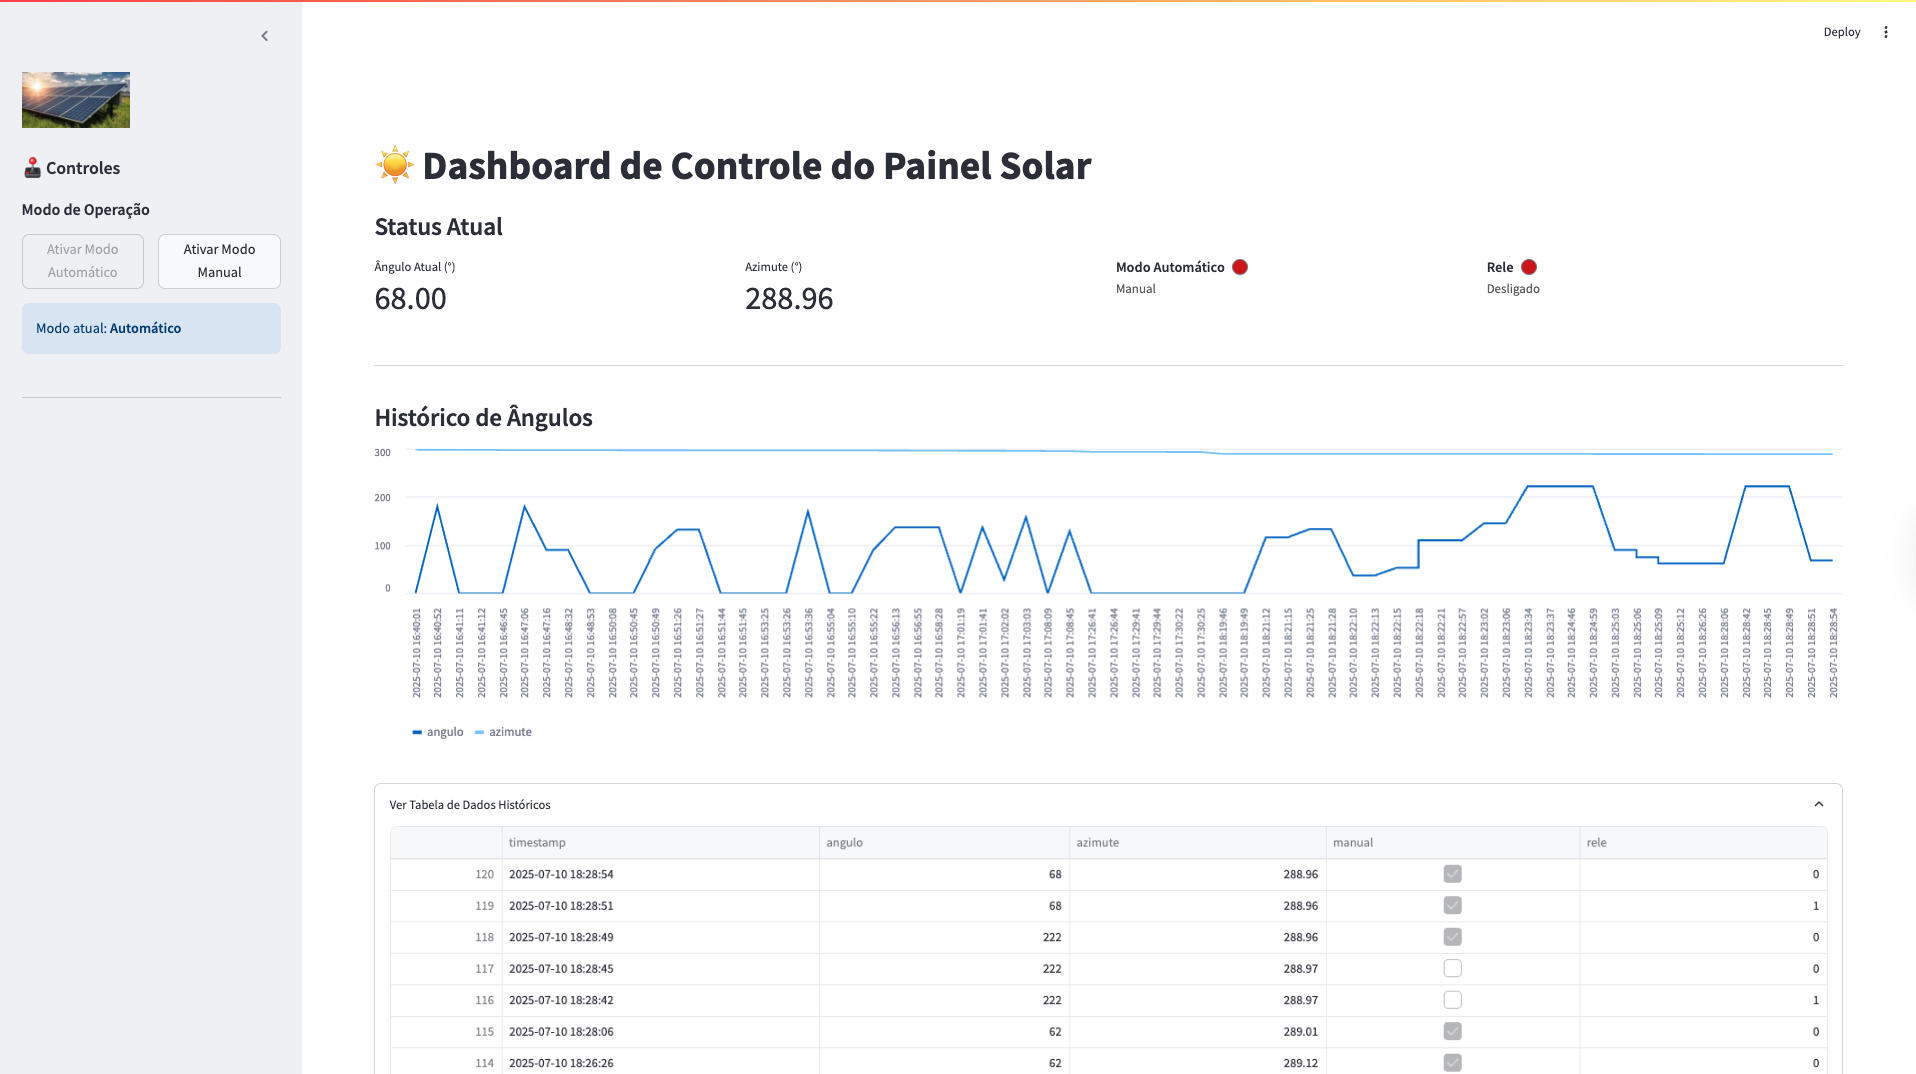
\includegraphics[width=0.9\textwidth]{tela_modo_automatico.png}
    \caption{Interface do dashboard no modo automático.}
    \label{fig:tela_automatico}
\end{figure}

\begin{figure}[H]
    \centering
    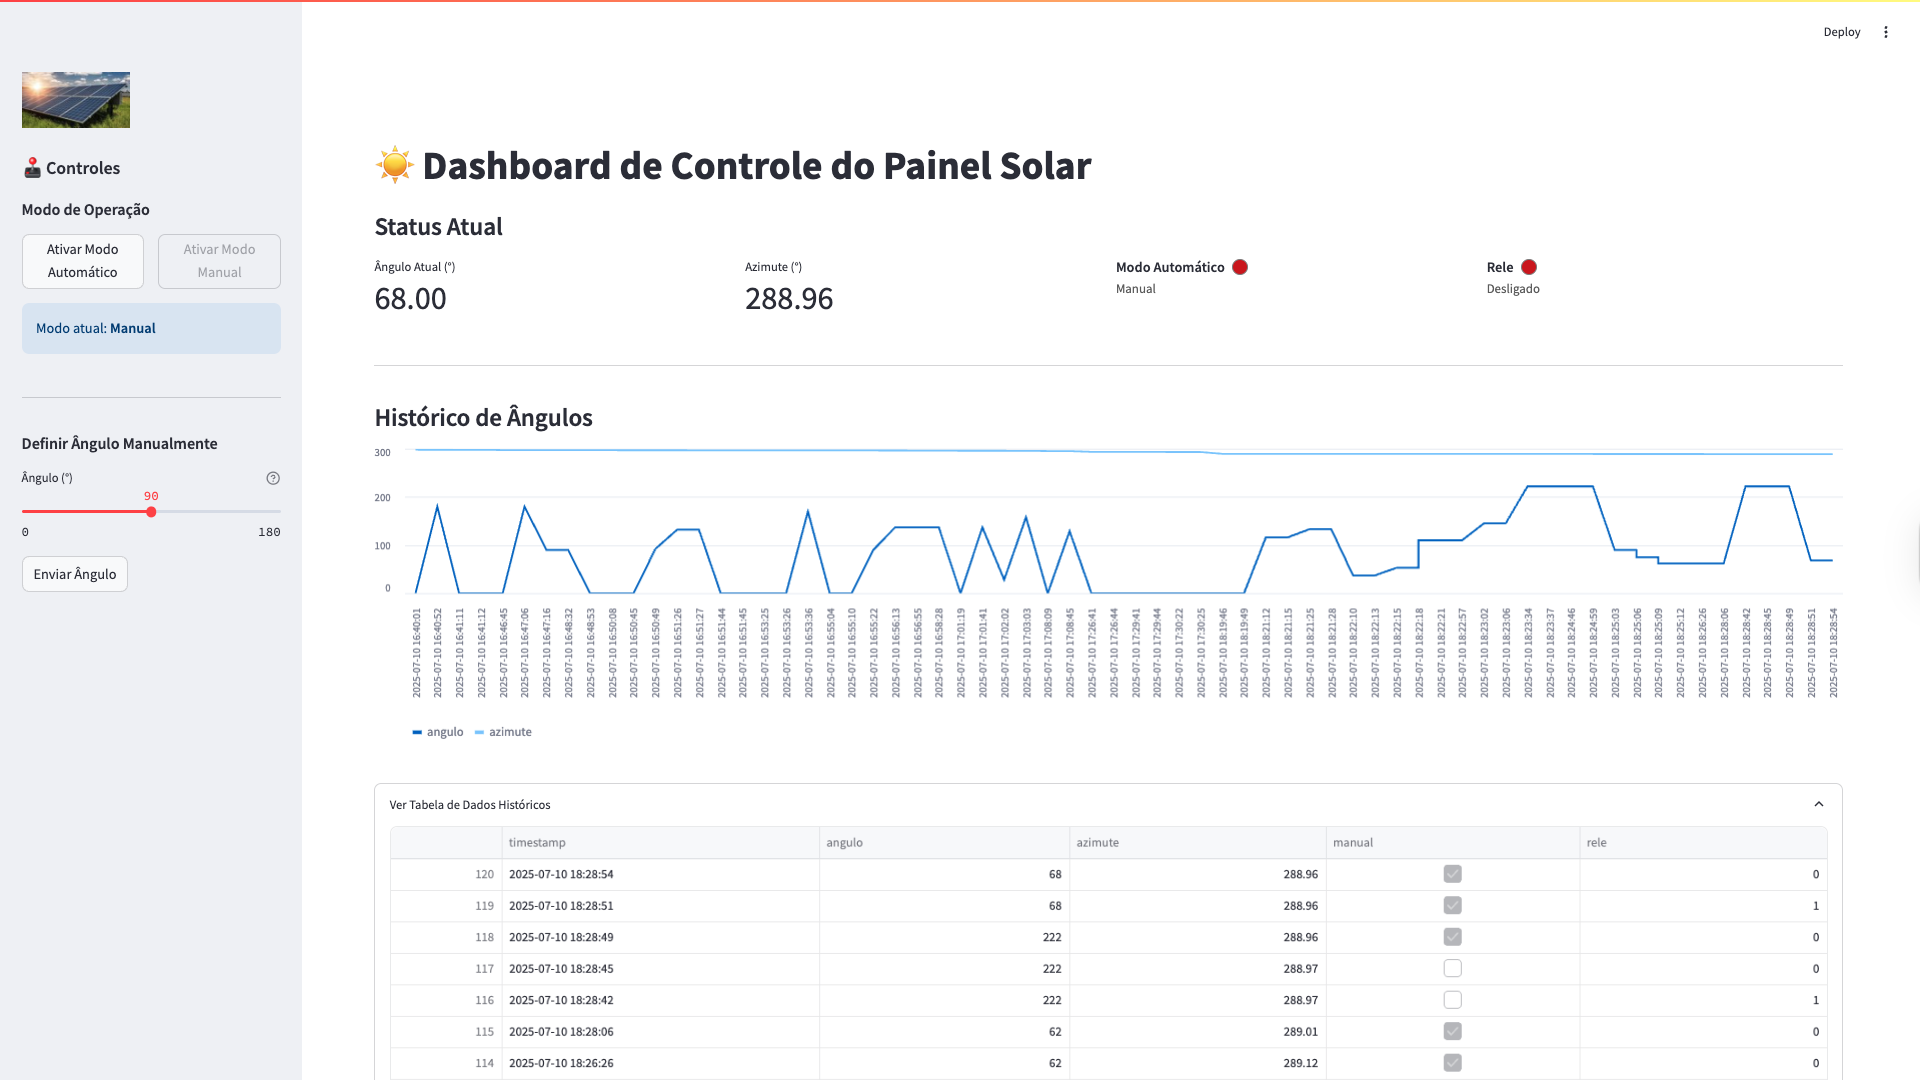
\includegraphics[width=0.9\textwidth]{tela_modo_manual.png}
    \caption{Interface do dashboard no modo manual, com o controle de ângulo visível na barra lateral.}
    \label{fig:tela_manual}
\end{figure}

\section{Conclusão}
% Conteúdo a ser adicionado futuramente.

\end{document}
